\chapter{Uitwerken Prototype ARCore}
\label{ch:prototype}

Dit hoofdstuk bevat een omschrijving van het uitgewerkte prototype. Het prototype bestaat uit verschillende grote delen die elk besproken worden in een aparte sectie. Het uitgewerkte prototype is te vinden op \href{https://github.com/MatthiasDeFre/Bachelorproef-Prototype}{de repository van het prototype} \autocite{GITHUBPROTOTY}.

\section{Unity Asset Store}
Unity beschikt over een Asset Store die developers, designers en zelfs muzikanten kunnen gebruiken om hun werk te delen met anderen. De assets op deze store kunnen andere developers dan gebruiken in hun projecten. Voor de ontwikkeling van het proptype zijn volgende assets gebruikt:

\begin{itemize}
    \item ZoneUI \autocite{MichskyZone}
    \item Clean Title Transitions \autocite{MichskyTitle}
    \item EnhancedScroller \autocite{EchoScroller}
    \item DoozyUI \autocite{DoozyUI}
    \item Plank Textures PBR \autocite{UnityWood}
\end{itemize}

\section{Hoofdmenu}
Wanneer de gebruiker de applicatie opstart komt hij op de hoofdpagina (zie figuur \ref{fig:prototypeUi}) terecht. Op deze pagina heeft hij verschillende opties waaruit hij kan kiezen. Als het de gebruiker zijn eerste keer is dat hij de applicatie gebruikt zullen alleen de opties 'Nieuw Levensverhaal' en 'Oude Levensverhalen bekijken (archief)' beschikbaar zijn. Indien de gebruiker toch al eens de applicatie heeft opgestart kan hij verder doen met zijn recentste levensverhaal of kiezen uit één van zijn niet voltooide levensverhalen. 

Vanuit het hoofdmenu heeft de gebruiker ook nog de optie om naar de instellingenpagina te gaan of naar zijn profielpagina. Op de gebruiker zijn profiel staan verschillende weetjes zoals het aantal deelgenomen levensverhalen, voltooide raadsels en ontdekte schilderijen. Ook heeft de gebruiker een level dat berekent is aan de hand van deze variabelen. Het behalen van een bepaald level is momenteel puur visueel en zit in de applicatie om de gebruiker een gevoel van trots en prestatie te geven.

\begin{figure}
    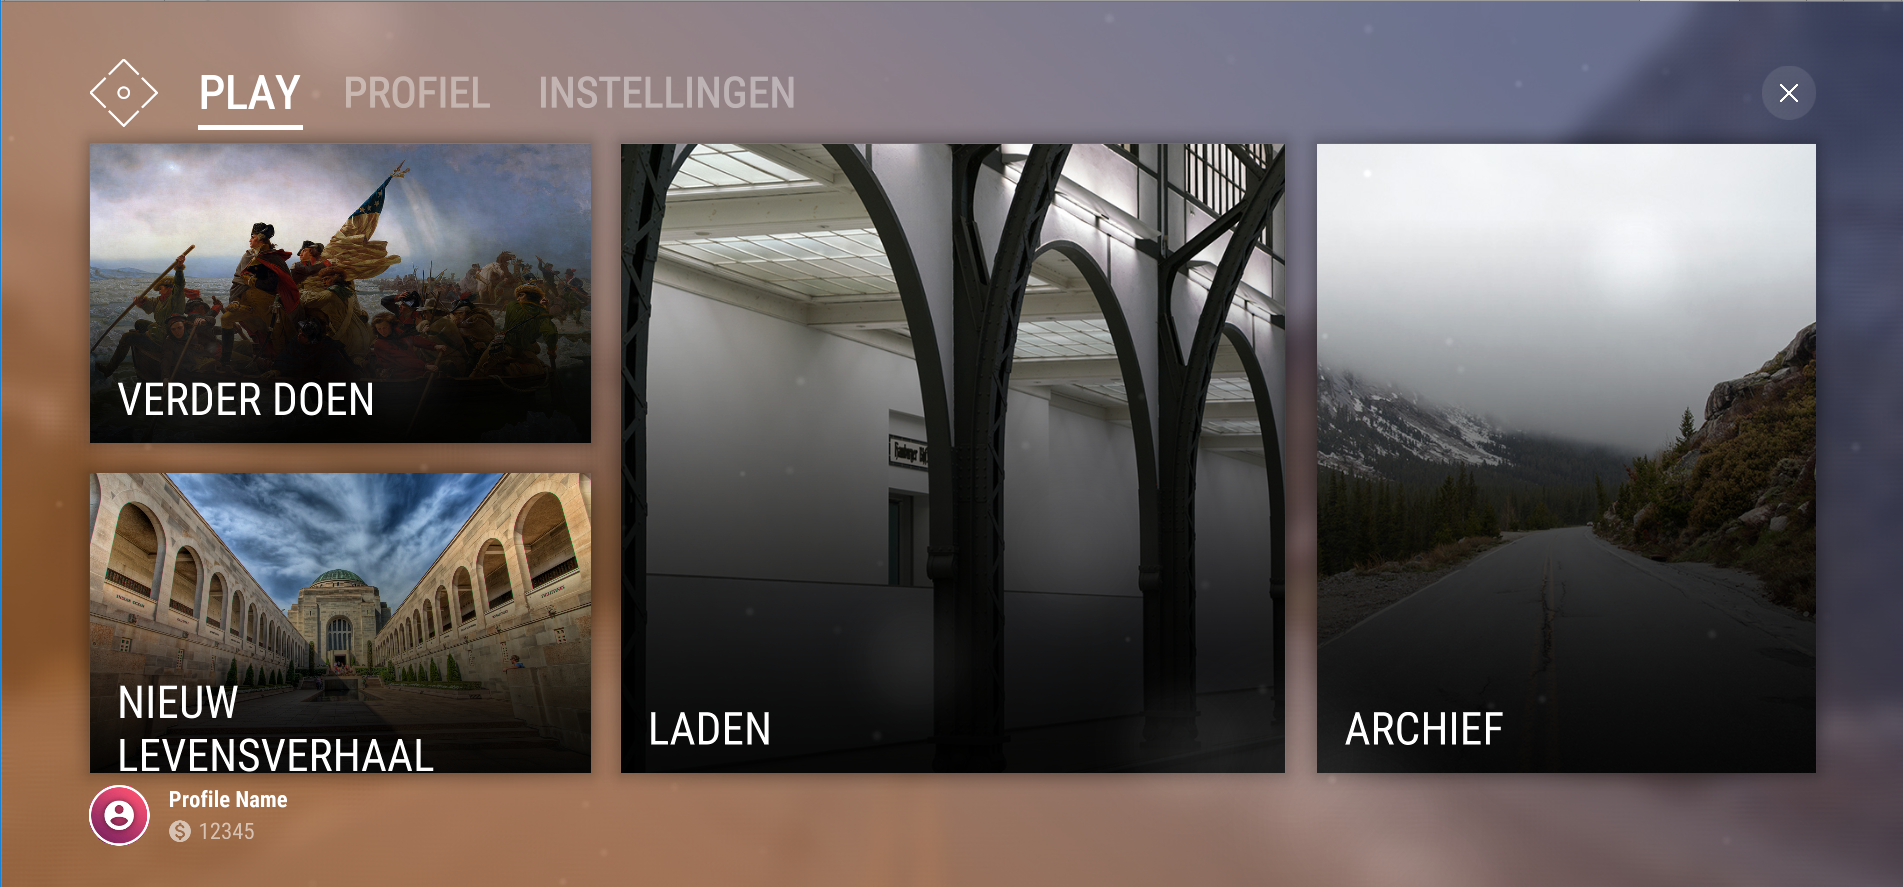
\includegraphics[width=\linewidth]{prototypeUi.png}
    \caption{Het hoofdmenu}
    \label{fig:prototypeUi}
\end{figure}
% + 1 If you get the reference

\section{Nieuw Levensverhaal Starten}
De gebruiker heeft de optie om een nieuw levensverhaal op te starten. Wanneer hij voor deze optie kiest krijgt hij een lijst van alle beschikbare levensverhalen. Deze lijst is niet hardcoded in de applicatie. Bij het opstarten zal de applicatie de lijst ophalen van een backendserver. Wanneer de gebruiker kiest voor levensverhaal moet de applicatie wel nog de concrete data ophalen van dit levensverhaal. Deze data is van het JSON datatype en bevat:

\begin{enumerate}
    \item Informatie over het levensverhaal
    \item Raadsels gelinkt aan het levensverhaal
    \item De benodigde afbeeldingen
\end{enumerate}

Door het levensverhaal op deze manier op te slaan is het makkelijk voor musea om nieuwe verhalen te creëren via een webinterface en deze direct beschikbaar te stellen voor de gebruiker. Omdat de afbeeldingen niet op voorhand beschikbaar zijn moet ARCore de image database tijdens het lopen van de applicatie creëren. Het toevoegen van een image 'at runtime' duurt ongeveer 30ms (wat niet lang is) en zolang het creëren van deze database op een ander thread gebeurt kan de gebruiker nog steeds de UI gebruiken. De applicatie slaat deze afbeeldingen op wat ervoor zorgt dat de gebruiker ze niet opnieuw moet downloaden indien hij hetzelfde levensverhaal een tweede keer wil beleven. 

Tijdens het downloaden en toevoegen aan de database krijgt de gebruiker een ladingscherm te zien dat info geeft over de huidige status van dit proces (zie figuur \ref{fig:loading}).
\begin{figure}
    
\includegraphics[width=\linewidth]{loading.png}
    \caption{Afhankelijk van het aantal gedownloade images / toegevoegd aan de database zal de ladingbalk zich vullen}
    \label{fig:loading}
\end{figure}

\subsection{Verloop van een Levensverhaal}
Wanneer het levensverhaal geladen is kan de gebruiker aan de slag gaan. De gebruiker krijgt het eerste kunstwerk te zien dat hij moet inscannen. Bij het inscannen van het kunstwerk krijgt de gebruiker dan wat extra informatie over het kunstwerk en de persoon waarover het gaat. Ook krijgt hij het volgende kunstwerk te zien dat hij moet inscannen. Bij het inscannen van het volgende kunstwerk kunnen er nu meerdere dingen gebeuren:

\begin{enumerate}
    \item Het nieuwe kunstwerk is beschikbaar (zie figuur \ref{fig:paintingReveal})
    \item Het nieuwe kunstwerk is nog niet beschikbaar en de gebruiker moest eerst een raadsel oplossen (zie figuur \ref{fig:paintingLocked})
\end{enumerate}
\begin{figure}
    \centering
    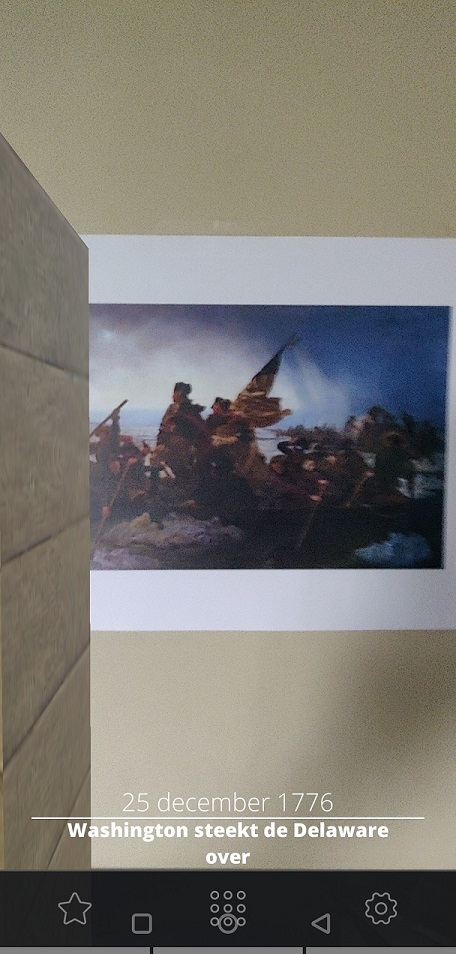
\includegraphics[width=\textwidth,height=\textheight,keepaspectratio]{paintingReveal.jpg}
    \caption{Het kunstwerk is ontgrendeld en toont zijn titel en datum}
    \label{fig:paintingReveal}
\end{figure}
\begin{figure}
      \centering
    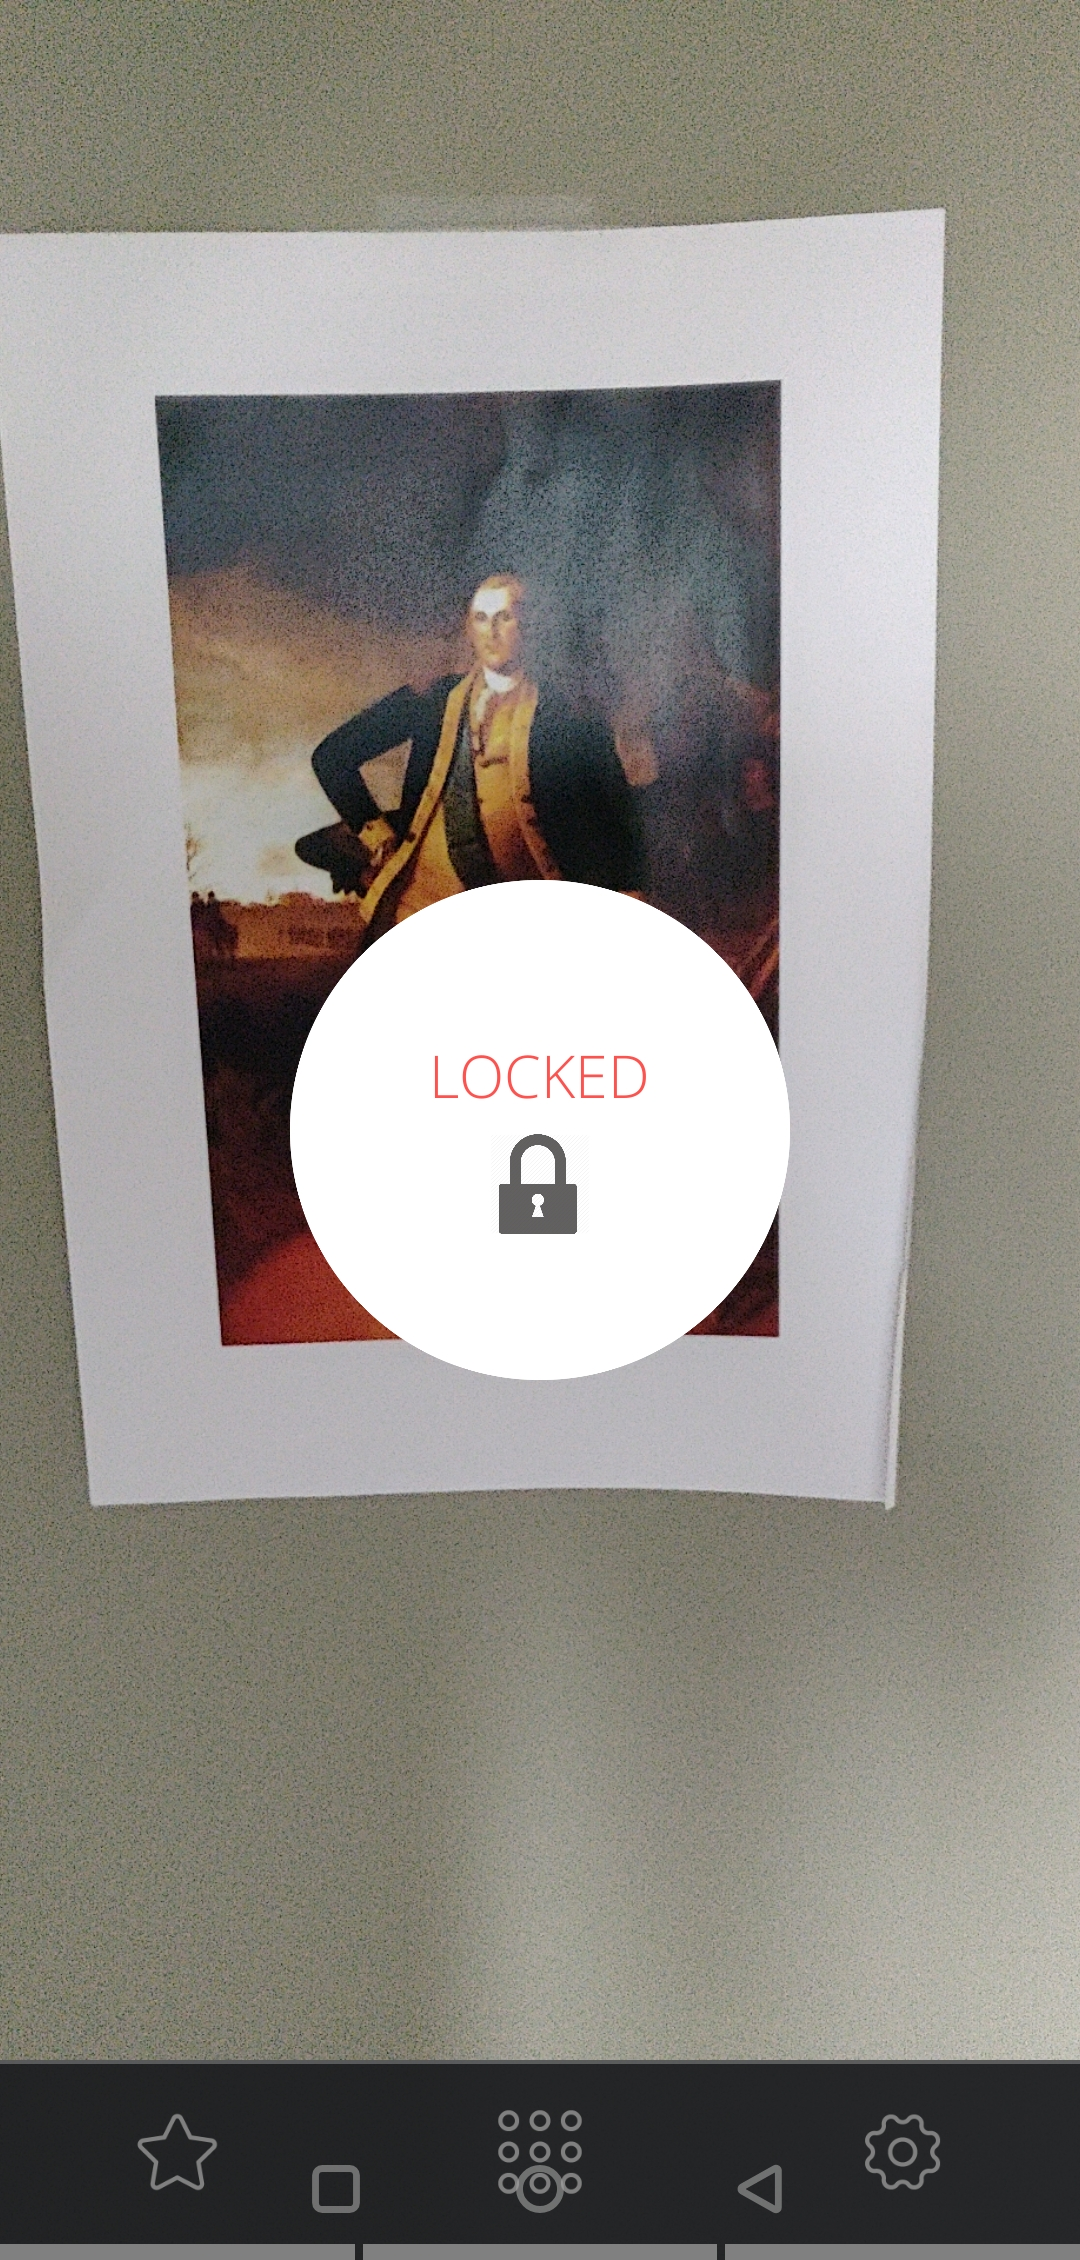
\includegraphics[width=\textwidth,height=\textheight,keepaspectratio]{paintingLocked.jpg}
    \caption{Het kunstwerk is vergrendeld en de gebruiker krijgt hierover een melding}
    \label{fig:paintingLocked}
\end{figure}


In het eerste geval zal de informatie over het kunstwerk ernaast verschijnen (zie figuur \ref{fig:paintingInfo}) en kan de gebruiker verder gaan naar het volgende kunstwerk. Bij het tweede geval moet de gebruiker iets extra doen om het volgende kunstwerk te kunnen scannen. Deze raadsels kunnen van verschillende vormen aannemen waaronder:

\begin{enumerate}
    \item Antwoorden van een vraag
    \item Opzoek gaan naar een item in een voorafgaand kunstwerk
    \item Opzoek gaan naar een item in het huidige kunstwerk
\end{enumerate}
\begin{figure}
    \centering
    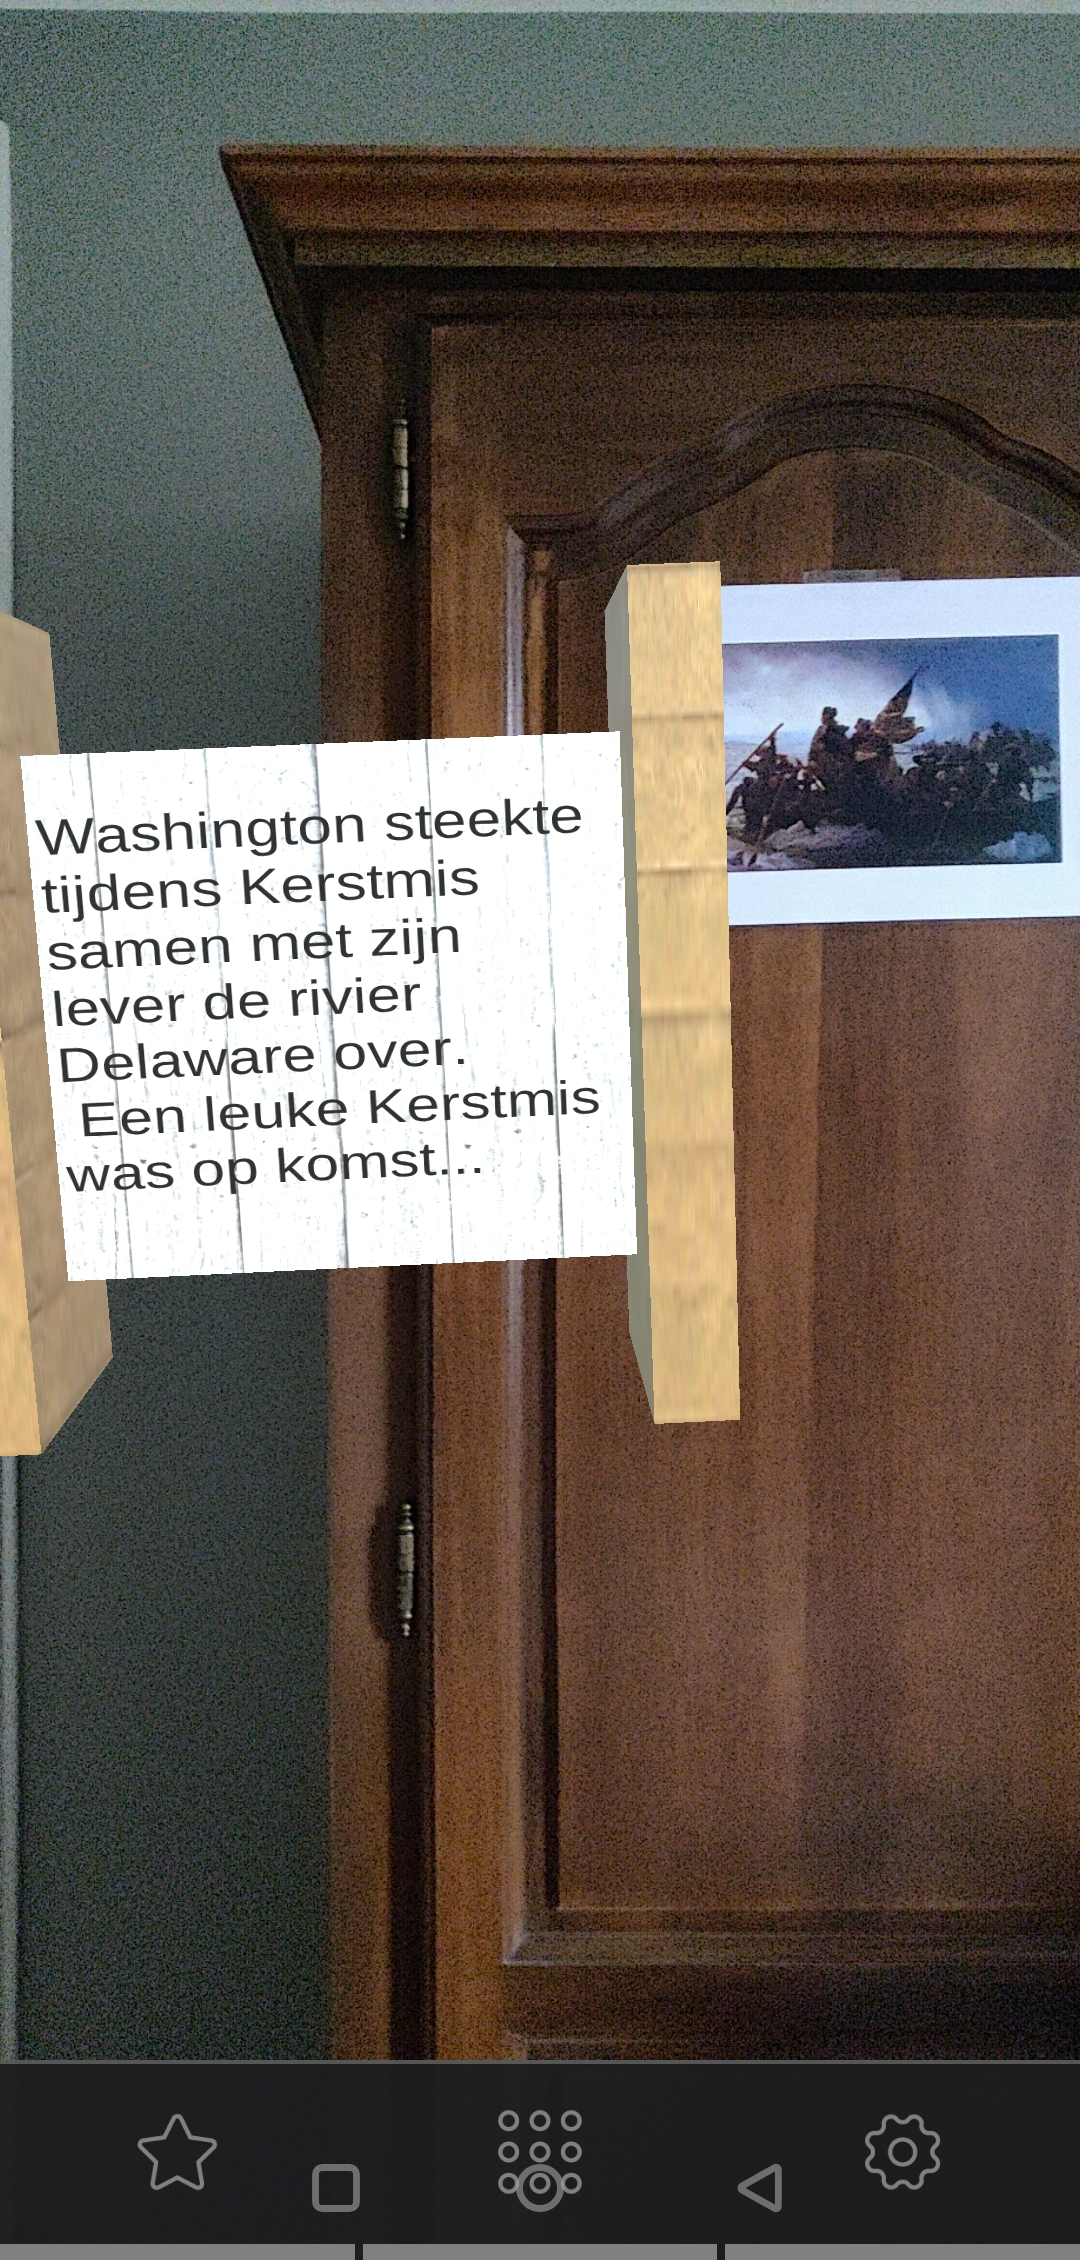
\includegraphics[width=\textwidth,height=\textheight,keepaspectratio]{paintingInfo.jpg}
    \caption{De informatie over het kunstwerk wordt ernaast getoond}
    \label{fig:paintingInfo}
\end{figure}
Deze cyclus blijft verder gaan tot de gebruiker het hele levensverhaal heeft ontdekt.

\subsection{Lijst van Kunstwerken}
Als de gebruiker wilt zien hoe ver hij exact in het levensverhaal zit kan hij de lijst van kunstwerken openen. Voor elk kunstwerk dat hij ontgrendeld heeft kan hij de afbeeldingen zien, indien hij het kunstwerk ook al gescand heeft kan hij ook de informatie hierover zien. Wanneer het kunstwerk nog vergrendeld is zal de gebruiker wel hints over de raadsels zien die uitleggen hoe hij het kunstwerk kan ontgrendelen.

Deze lijst maakt gebruik van de EnhancedScroller Asset van \textcite{EchoScroller} omdat deze veel performanter is dan de standaard lijst in Unity. De EnhancedScroller maakt gebruik van het RecyclerView principe. Dit betekent dat alleen de data van de kunstwerken waarvan de indexen (inclusief een paar extra boven- en onderaan) zichtbaar zijn ingeladen is. Hierdoor zijn heel grote levensverhalen met veel kunstwerken ook mogelijk.

\subsection{Het Plaatsen van een Eigen Museum}
De gebruiker heeft ook de optie om een soort van eigen museum the plaatsen in de echte wereld. Door een virtuele muur in de echte wereld te plaatsen heeft de gebruiker de mogelijkheid om hierop ontgrendelde kunstwerken, informatie of hints van raadsels te plaatsen (zie figuur \ref{fig:paintingGallery}). Deze functionaliteit is vooral ontwikkelt voor grote musea waarbij de kunstwerken verder uit elkaar hangen. Wanneer een gebruiker weet dat hij naar kunstwerk X moet gaan om daar een raadsel op te lossen zal hij eens hij daar is misschien niet meer weten wat hij exact moest doen. De gebruiker kan natuurlijk ook gewoon de lijst van schilderijen openen om daar te kijken wat hij exact moet doen, maar op deze manier kan de hele ervaring augmented blijven.

\begin{figure}
    \centering
    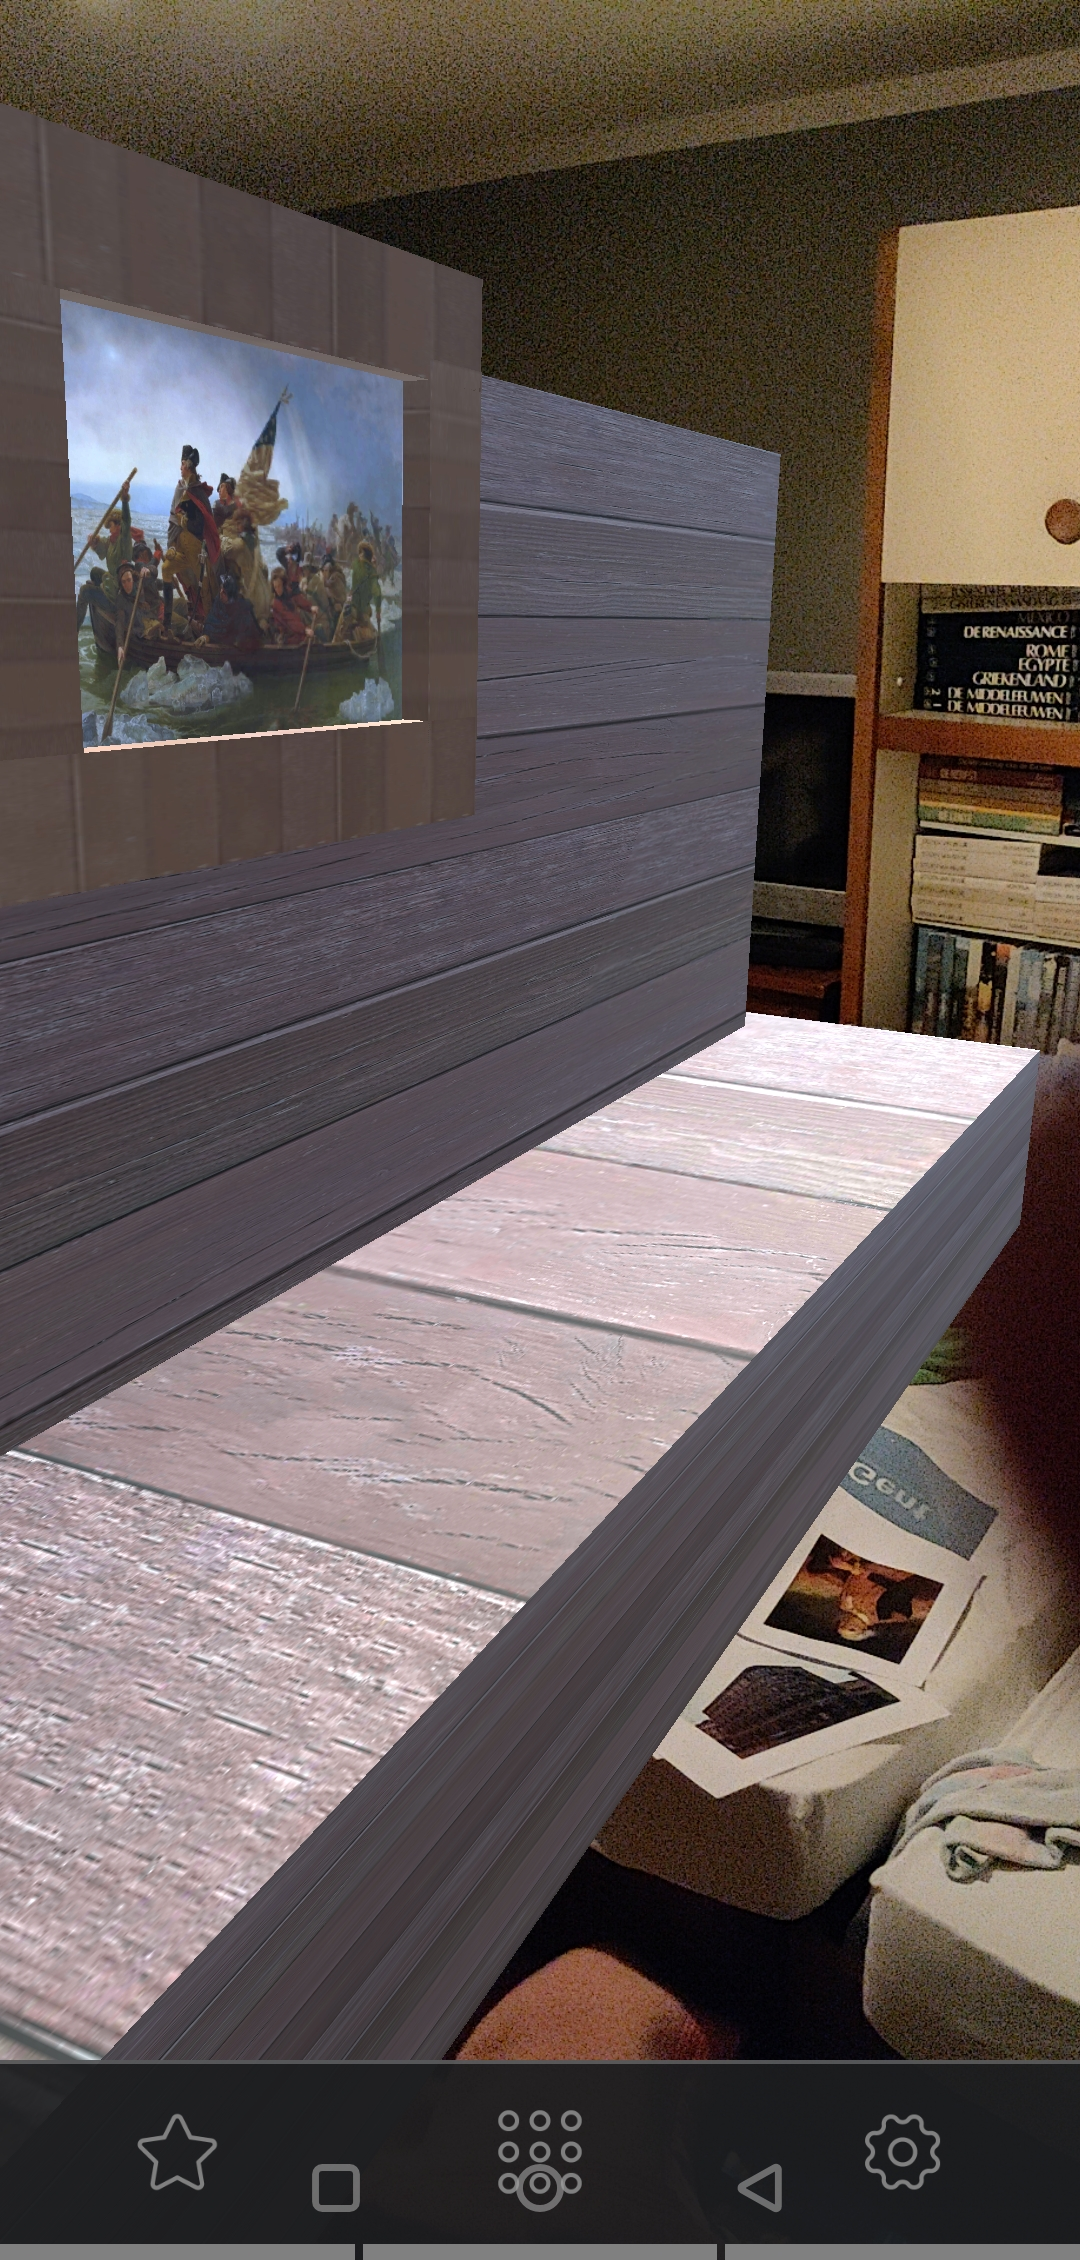
\includegraphics[width=\textwidth,height=\textheight,keepaspectratio]{paintingGallery.jpg}
    \caption{Een geplaatste galerij waarop de gebruiker zijn ontgrendelde schilderijen op kan plaatsen}
    \label{fig:paintingGallery}
\end{figure}

\section{Lijst van Levensverhalen}
In dit scherm bevinden zich alle levensverhalen die ooit hebben bestaan zelf als de gebruiker er niet aan heeft meegedaan. Op deze manier gaat het werk van het museum nooit verloren. De gebruikers kunnen hier een levensverhaal selecteren en de informatie over de kunstwerken lezen. Ook is er de optie om zelf de schilderijen af te drukken waardoor de gebruikers ook de mogelijkheid hebben om bij hun thuis de tentoonstelling uit te voeren.